\subsection{Binary call at the money}\lesson{5}{19/03/2020}
We consider, as an example, the binary call at the money. In this case, the payoff is 
\begin{equation}
    \mbox{payoff}_T = \mathds{1}_{S_T\ge K}
\end{equation}
and $K=S_0$ (at the money). So, when it is possible to exercise the contract, the cash flow is always equal to 1. Consider a toy model with $u=1.1$, $d=0.9$ and $S_0=K=100$:
\begin{center}
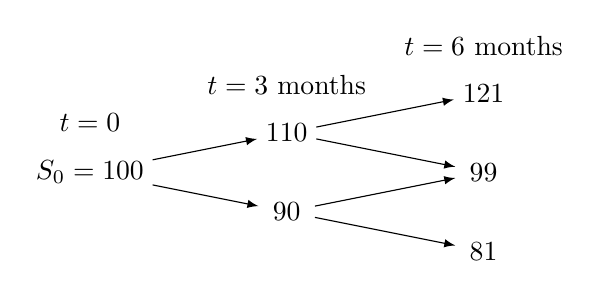
\begin{tikzpicture}[
                   grow = right,
edge from parent/.style = {draw,-latex},
         label distance = 1.5mm,
      every node/.style = {minimum width=2em, inner sep=3pt},
         level distance = 25mm,
       sibling distance = 10mm,
                     ]
\node[label=90:{$t=0$}] {$S_0=100$}
    child {node {90}
        child {node {81}
            %child {node {40}}
            %child {node {20}}
                }
        child {node {}}%<---------------- already printed
            }
    child {node[label=90:{$t=3$ months}] {110}
        child {node {99}
            %child {node {}}%<------------ already printed
            %child {node {0}}
                }
        child {node[label=90:{$t=6$ months}] {121}
            %child {node {}}%<------------ already printed
            %child {node[label=90:{$t=3$}] {0}}
                }
                };
\end{tikzpicture}
\end{center}
The payoff is 
\begin{equation}
    \mbox{payoff}_T = 
    \left( 
    \begin{matrix}
    1 \\ 0 \\ 0
    \end{matrix}
    \right)
\end{equation}
We would like to price this option. The input are the zero coupon bonds at these maturities:
\begin{enumerate}
    \item The first has notional value 1 at 3 months and 
    its price today is 1.001. 
    \begin{equation*}
        1.001 = e^{-R(0,3m)\frac{3}{12}}\cdot1 \qquad\Rightarrow\qquad R(0,3m) = -0.001 = -0.1\%
    \end{equation*}
    This means that the interest rate is negative and it is as if we pay in order to keep our money safe.
    \item The second has notional value 1 at 6 months an its price today is 1, so the interest rate is zero.
\end{enumerate}
In order to find which is the forward interest rate, we use eq. \eqref{equality}:
\begin{equation}\label{equality1}
    e^{R\left(0,3m\right)\frac{3}{12}}e^{R\left(0,3m,6m\right)\frac{3}{12}} = e^{R(0,6m)\frac{6}{12}}
\end{equation}
which has solution
\begin{equation}
    R\left(0,3m,6m\right) = 2\underbrace{R(0,6m)}_{=0}-R\left(0,3m\right) = 0.1\%
\end{equation}
Therefore, the risk neutral probability weights are given by
\begin{equation}
    q_1 = \dfrac{e^{R\left(0,3m,6m\right)\frac{3}{12}}-d}{u-d} = 4.501, \qquad q_0 = \dfrac{e^{R\left(0,3m\right)\frac{3}{12}}-d}{u-d} = 4.499
\end{equation}
Now we are able to price the corresponding binary option:
\begin{equation}
    price_0^{BinCall} = e^{-RT}\mathbb{E}^{\Qmeas}[\mbox{payoff}_T] = e^{-RT}\mathbb{E}^{\Qmeas}\left[
    \left( 
    \begin{matrix}
    1 \\ 0 \\ 0
    \end{matrix}
    \right)
    \right]
\end{equation}
where
\begin{equation}
    Q \sim \left(
    \begin{matrix}
    q_0q_1 \\ (1-q_0)q_1+q_0(1-q_1) \\ (1-q_0)(1-q_1)
    \end{matrix}
    \right)
\end{equation}
which gives
\begin{align}
    \notag price_0^{BinCall} 
    &= 
    \notag e^{-R(0,6m)\frac{6}{12}}(1\cdot q_0q_1 + 0\cdot (1-q_0)q_1+q_0(1-q_1) + 0\cdot (1-q_0)(1-q_1)) \\
    &=
    e^{-R(0,6m)\frac{6}{12}}q_0q_1
\end{align}
For the hedging the story is the same. \colorbox{cyan}{scrivi}

\section{General binomial model}
Now we consider a generic number of time steps, so that the underlying is $S_T\in\mathbb{R}^{t+1}$ and has terminal value
\begin{equation}
    \left(
    \begin{matrix}
    Su^t \\ Su^{t-1}d \\ \vdots \\ Su^jd^{t-j} \\ \vdots \\ Sud^{t-1} \\ Sd^t
    \end{matrix}
    \right)
\end{equation}
where $j$ represents the number of up moves in the lattice. The payoff (for the call option) we want to compute is 
\begin{equation}
    \mbox{payoff}_T = (S_T-K)^+
\end{equation}
Then the value of the corresponding replicating portfolio is
\begin{align}
    \notag P_t(j) 
    &=
    \notag V_t(j) \overset{(a)}{=} e^{-R\cdot1}(qV_{t+1}(j+1) + (1-q)V_{t+1}(j)) \\
    &=
    e^{-R}\mathbb{E}^{\Qmeas}[V_{t+1}|j]
\end{align}
% forse ha usato V per indicare "value", ma crea confusione quindi forse è meglio usare sempre P
where in (a) we used the backward induction procedure using unitary time steps and constant $q=\frac{e^R-d}{u-d}$. At the end, the corresponding value is
\begin{equation}
    P_T(j) = (S_0u^jd^{T-j}-K)^+
\end{equation}
Considering the hedging, we have
\begin{equation}
    \Delta_t(j)=\dfrac{V_{t+1}(j+1)-V_{t+1}(j)}{S_tu-S_td}, \qquad \beta_t(j)=e^{-Rt}(V_t(j)-\Delta_t(j)S_t) 
\end{equation}
So the initial price can be written as:
\begin{equation}
    p_0(call)=e^{-RT}\sum^{T}_{j=0}\binom{T}{j}q^j(1-q)^{T-j}(Su^j d^{T-j}-K)^+
\end{equation}
\begin{remark}
    Notice that the probability distribution
    \begin{equation}
        Q \sim \left(
        \begin{matrix}
        q^T \\ \vdots \\ \binom{T}{j}q^j(1-q)^{T-j} \\ \vdots \\ (1-q)^T
        \end{matrix}
        \right)
    \end{equation}
    is normalized, in fact
    \begin{equation}
        \sum^{T}_{j=0}\binom{T}{j}q^j(1-q)^{T-j} = (q+1-q)^T = 1
    \end{equation}
    where we used the fact that $(a+b)^n=\sum^{n}_{j=0}\binom{n}{j}q^j(1-q)^{n-j}$.
\end{remark}


\section[Convergence of the binomial model]{From the binamial model to a geometric brownian motion}
Now we want to see if the binomial model leads to convergence if we take a number of steps which tends to infinity. Let's consider a binomial model with unitary time steps, $n<T$ and $T=m$. The underlying at time $n+1$ is defined as
\begin{equation}\label{Sn+1}
    S_{n+1} = S_nZ_{n+1}
\end{equation}
where $Z_n$ are i.i.d. random variables with binomial distribution and risk neutral probability
\begin{equation}
    Q(Z_{n+1}=u_n)=q_n, \qquad Q(Z_{n+1}=d_n)=1-q_n
\end{equation}
with 
\begin{equation}
    q_n = \dfrac{e^R-d_n}{u_n-d_n}
\end{equation}
In principle, if we consider this particular binomial model and we consider the discounted asset $S_ne^{-Rn}$, it turn out to be a $Q$-martingale, i.e. a martingale under the measure ${\Qmeas}$. This means that $S_ne^{-Rn}$ is constant in expected value and that
\begin{equation}
    \mathbb{E}^{\Qmeas}[Z_n] = e^{R\frac{T}{n}}
\end{equation}
In order to prove it, it is sufficient to start from eq. \eqref{Sn+1} \colorbox{cyan}{to do (6:50)}.\\
We would like to shift from the multiplicative structure of \eqref{Sn+1} to an additive structure. This can be done just by taking the logarithm of eq. \eqref{Sn+1}:
\begin{equation}\label{lnSn}
    \ln S_n = \ln S_0 + \sum_{i=1}^n\ln Z_i
\end{equation}
The sum in \eqref{lnSn} is a sum of bounded i.i.d random values, so we can use the Central Limit Theorem in order to show that it converges to a gaussian random variable. However, the convergence is not well defined as $\low(\ln Z_i)$ depends on $n$ and when the random variable depends on the number of random variables considered we have to be careful in considering the limit. So we can not use a simple version of the CLT. The idea is to show that 
\begin{equation}
    \low(S_n)\to\low(S_T)
\end{equation}
where $S_T$ is the terminal value of a process $S_t$ satisfying
\begin{equation}\label{geom_brow}
    \dv{S_t}{t} = r\dd t + \sigma\dd W^{\Qmeas}_t
\end{equation}
where $W^{\Qmeas}_t$ is a brownian motion under the probability measure ${\Qmeas}$. In order to study the convergence it is better to work with the corresponding characteristic function, which is the Fourier transform of the pdf:
\begin{align}\label{phi111}
    \notag \phi_{\ln S_n}(\lambda)
    &=
    \mathbb{E}^{\Qmeas}[e^{i\lambda\ln S_n}] \overset{\eqref{lnSn}}{=} e^{i\lambda\ln S_0}\left(\mathbb{E}^{\Qmeas}\left[e^{i\lambda\ln Z}\right]\right)^n \\
    &= S_0^{i\lambda}\left(qe^{i\lambda\ln n}+(1-q)e^{i\lambda\ln d}\right)^n
\end{align}
Now we define the relation between $(u,d)$ and $(r,\sigma)$. Let's take
\begin{equation}\label{undn}
    u_n=e^{\sigma\sqrt{\frac{T}{n}}}, \qquad d_n=e^{-\sigma\sqrt{\frac{T}{n}}}
\end{equation}
which is in line with what we did in sec. \ref{sec:impl}. Now we have to link the interest rate for the period in the binomial model with the corresponding interest rate in the continuous time version:
\begin{equation}\label{Rr}
    e^R = e^{r\frac{T}{n}}
\end{equation}
where $R$ is the discrete time interest rate and $r$ is the continuous time interest rate. Plugging this mapping in \eqref{phi111} we get:
\begin{align}\label{phi222}
    \notag \phi_{\ln S_n}(\lambda) 
    &=
    S_0^{i\lambda}\left(qe^{i\lambda\sigma\sqrt{\frac{T}{n}}}+(1-q)e^{-i\lambda\sigma\sqrt{\frac{T}{n}}}\right)^n \\
    &\overset{(a)}{=}
    \notag S_0^{i\lambda}\left[q
    \left(
    1+i\lambda\sigma\sqrt{\frac{T}{n}}-\frac{1}{2}\lambda^2\sigma^2\frac{T}{n}+\order{n^{-1}}
    \right) + \right. \\
    &\notag\qquad
    \left.+(1-q)\left(
    1-i\lambda\sigma\sqrt{\frac{T}{n}}-\frac{1}{2}\lambda^2\sigma^2\frac{T}{n}+\order{n^{-1}}
    \right)
    \right]^n \\
    &= 
    S_0^{i\lambda}\left(1+i\lambda\sigma\sqrt{\frac{T}{n}}(2q-1)-\frac{1}{2}\lambda^2\sigma^2\frac{T}{n}+\order{n^{-1}}\right)^n
\end{align}
where in (a) we used the Taylor expansion. Now, recall that $q = \frac{e^R-d}{u-d}$, so using \eqref{undn}, \eqref{Rr} and Taylor expanding we get
\begin{align}
    \notag q 
    &=
    \dfrac{e^{r\frac{T}{n}}-e^{-\sigma\sqrt{\frac{T}{n}}}}{e^{\sigma\sqrt{\frac{T}{n}}}-e^{-\sigma\sqrt{\frac{T}{n}}}} \\
    &= 
    \notag \dfrac{1+r\frac{T}{n}-1+\sigma\sqrt{\frac{T}{n}}-\frac{1}{2}\sigma^2\frac{T}{n}+\order{n^{-1}}}{1+\sigma\sqrt{\frac{T}{n}}+\frac{1}{2}\sigma^2\frac{T}{n}-1+\sigma\sqrt{\frac{T}{n}}-\frac{1}{2}\sigma^2\frac{T}{n}+\order{n^{-1}}} \\
    &=
    \notag \dfrac{\sigma+\left(r-\frac{\sigma^2}{2}\right)\sqrt{\frac{T}{n}}+\order{n^{-1/2}}}{2\sigma+\order{n^{-1/2}}} \\
    &=
    \frac{1}{2}+\dfrac{1}{2\sigma}\left(r-\frac{\sigma^2}{2}\right)\sqrt{\frac{T}{n}}+\order{n^{-1/2}}
\end{align}
Then we have
\begin{equation}
    2q-1 = \dfrac{1}{\sigma}\left(r-\frac{\sigma^2}{2}\right)\sqrt{\frac{T}{n}}+\order{n^{-1/2}}
\end{equation}
and we can plut it into \eqref{phi222}:
\begin{align}\label{phi333}
    \notag \phi_{\ln S_n}(\lambda) 
    &=
    \notag S_0^{i\lambda}\left(1+i\lambda\cancel{\sigma}\left(r-\frac{\sigma^2}{2}\right)\cancel{\frac{1}{\sigma}}\frac{T}{n}-\frac{1}{2}\lambda^2\sigma^2\frac{T}{n}+\order{n^{-1}}\right)^n \\
    &= 
    S_0^{i\lambda}\left[1+\frac{1}{n}\left(
    i\lambda T\left(r-\frac{\sigma^2}{2}\right)-\frac{1}{2}\lambda^2\sigma^2 T\right)\right]^n
\end{align}
Recall that 
\begin{equation*}
    \lim_{n\to+\infty}\left(1+\dfrac{a}{n}\right)^n = e^a
\end{equation*}
so if in \eqref{phi333} we define $a = \left(i\lambda T\left(r-\frac{\sigma^2}{2}\right)-\frac{1}{2}\lambda^2\sigma^2 T\right)$, we have that 
\begin{equation}\label{lim_phi}
    \lim_{n\to+\infty} \phi_{\ln S_n}(\lambda) = S_0^{i\lambda}\exp\left[i\lambda T \left(r-\frac{\sigma^2}{2}\right)-\frac{1}{2}\lambda^2\sigma^2 T \right]
\end{equation} 
Now we have to understand how \eqref{lim_phi} is related to the characteristic function of the terminal value of $\ln S_T$ in the continuous time framework, $\mathbb{E}^{\Qmeas}\left[e^{i\lambda\ln S_T}\right]$. We will find that the solution of \eqref{geom_brow} is 
\begin{equation}
    S_T = S_0e^{\left(r-\frac{\sigma^2}{2}\right)T+\sigma W_T^{\Qmeas}}
\end{equation}
$W_T^{\Qmeas} \sim \mathcal{N}(0;T)$ so the brownian motion has a gaussian distribution with variance equal to the time window we are considering. This means that $S_T$ is a random variable distributed as 
\begin{equation}\label{ST}
    S_T\sim S_0\exp\left[\underbrace{\ln S_0+\left(r-\frac{\sigma^2}{2}\right)T}_{deterministic}+\underbrace{\sigma\mathcal{N}(0;T)}_{stochastic}\right]
\end{equation}
The deterministic part represents just a shift in the expected value, so we can rewrite \eqref{ST} as
\begin{equation}
    S_T\sim S_0\exp[\sigma\mathcal{N}\left(\ln S_0+\left(r-\frac{\sigma^2}{2}\right)T;\sigma^2 T\right)]
\end{equation}
So $S_T$ follows a log-normal distribution. Now recall the characteristic function of a gaussian variable
\begin{equation}
    \mathbb{E}^{\Qmeas}\left[e^{i\lambda\mathcal{N}(\mu;\sigma^2)}\right] = e^{i\lambda\mu-\frac{\sigma^2\lambda^2}{2}}
\end{equation}
In our case we have:
\begin{align}
    \mathbb{E}^{\Qmeas}\left[e^{i\lambda\ln S_T}\right] 
    &=
    \mathbb{E}^{\Qmeas}\left[e^{i\lambda\mathcal{N}\left(\ln S_0+\left(r-\frac{\sigma^2}{2}\right)T;\sigma^2 T\right)}\right] \\
    &=
    \exp\left(i\lambda\ln S_0+i\lambda\left(r-\frac{\sigma^2}{2}\right)T-\dfrac{\sigma^2\lambda^2}{2}T\right) \\
    &=
    S_0^{i\lambda}\exp\left(i\lambda\left(r-\frac{\sigma^2}{2}\right)T-\dfrac{\sigma^2\lambda^2}{2}T\right)
\end{align}
This is the characteristic function of the geometric brownian motion. Going back to \eqref{lim_phi} we find exactly the same expression, so the binomial model converges to the characteristic function of the corresponding solution of the geometric brownian motion.